
\documentclass[12pt ]{iopart}
\usepackage{graphicx}
\usepackage{amsmath}
\usepackage[space]{grffile}
\usepackage{epstopdf}
\usepackage[autostyle,italian=guillemets]{csquotes}%bibliografia
%%\usepackage[bibstyle=authoryear,citestyle=authoryear-comp,backend=biber,uniquelist=false]{biblatex}%stile bibliografia
\usepackage[style=authoryear-icomp,maxbibnames=9,maxcitenames=1,uniquelist=false,
    backend=biber]{biblatex}

\usepackage{algorithm}
\usepackage[noend]{algpseudocode}

\addbibresource{b.bib}
%\newcommand{\gguide}{{\it Preparing graphics for IOP Publishing journals}}
%Uncomment next line if AMS fonts required
%\usepackage{iopams}  
\begin{document}

\title[DNN for EEG-fNIRS BCI]{Deep Learning for  hybrid EEG-fNIRS Brain Computer Interface: application to Motor Imagery Classification}

\author{Pierpaolo Croce\textsuperscript{1,2}, Filippo Zappasodi\textsuperscript{1,2}, Francesco di Pompeo\textsuperscript{1,2} Arcangelo Merla\textsuperscript{1,2} \& Antonio Maria Chiarelli\textsuperscript{1,2}}

\ead{pierpaolo.croce@unich.it}
\vspace{10pt}
\begin{indented}
\item[] \textsuperscript{1} Department of Neuroscience, Imaging and Clinical Sciences, "G.d’Annunzio" University, Chieti, Italy
\item[] \textsuperscript{2} Institute of Advanced Biomedical Technologies, "G.d’Annunzio" University, Chieti, Italy
\end{indented}

\begin{abstract}
	\\
	\textit{Objective.} to be filled. \\
	\textit{Approach.} to be filled.\\
	\textit{Main Results.} to be filled. \\
	\textit{Significance.} to be filled.
\end{abstract}


\section{Introduction}

Brain Computer Interface (BCI) refers to a group of procedures that directly link  central nervous system to a computer or a device [ref.]. BCI can focus on mapping, assisting, augmenting, or repairing human cognitive and sensory-motor functions. 
Historically, BCI was performed using Electroencephalography (EEG) [ref.]. EEG  provides information regarding brain electrical activity with very high temporal resolution (ms scale) [ref.]. 

In the last years, BCI studies investigated the possibility of combining EEG with other neuroimaging technologies [ref.]. Among these, functional Near Infrared Spectroscopy (fNIRS) provided encouraging results [ref.]. 

EEG and fNIRS are both flexible, scalp located procedures. Whereas EEG captures the macroscopic temporal dynamics of brain electrical activity through passive voltages evaluation, fNIRS estimates brain hemodynamic oscillations  relying on spectroscopic measurements of oxy- and deoxy-hemoglobin (HbO and Hb, respectively) fluctuations in the cortex [ref.]. Orthogonally with respect to EEG, fNIRS, depending on the slow dynamics of the hemodynamic response, yields low temporal resolution but, because of the fast exponential decay of light sensitivity, it provides good spatial resolution (around 1 cm) \parencite{chiarelli2016combining}. 

Because of different physiological information provided by and characteristic of EEG and fNIRS [ref. croce], higher BCI performances  of combined measurements with respect to standalone EEG were reported extensively [ref.] .

Two main processing steps are involved in BCI:  feature extraction and classification. 

EEG features are usually extracted based on the power of the signal frequency bands. Indeed, well-distinct behaviors of EEG signal have been identified based on signal frequencies (delta ($< 4 Hz$), theta ($4-7 Hz$), alpha ($8-15 Hz$), beta ($16-31 Hz$), and gamma ($> 31 Hz$) ref.]). For example, during the execution of a motor task (or during the imagination or observation of the movement), the beta activity is suppressed in related brain areas(Event Related Desynchronization, ERD)[ref.].  
fNIRS  features are generally  computed from  HbO and Hb variations in the brain which are dependent, among others, on the  Blood Oxygen Level Dependant (BOLD) effect [cit.]. 

The classification procedure aims to accurately classify the brain state  based on the extracted signal features  and it is a fundamental step of BCI processing.


Different  experiment and algorithms have been applied  to combined EEG-fNIRS BCI. \textcite{Fazli_2012} proposed Linear Discriminant Analysis to classify ERD EEG and time average fNIRS concentration changes during executed movements as well as motor imagery.  In \textcite{ma2012hybrid} a Gaussian radial-basis kernel Support Vector Machine (SVM) was used to classify a motor imagery BCI based on EEG power spectral densities and fNIRS amplitude of the cerebral blood oxygen signal.   \textcite{lee2014hybrid} employed LDA on combined EEG and fNIRS features to classify three conditions: right and left motor imagery and idle status . They reached a classification accuracy of about $65\%$. In \textcite{buccino2016hybrid} the features to be submitted to a LDA were extracted combining two methods: Regularized Common Spatial Patterns (RCSP) for EEG and combination of average and slope indicators for fNIRS signals. In this case an accuracy between $72-79\%$ was reached in a movement recognition task. In  \textcite{khan2014decoding, khan2017hybrid} LDA was used to classify control commands based on EEG peak amplitudes of selected motor area channels and mean values of HbO and Hb for fNIRS with accuracy ranging between $80-95\%$.
For all of the above mentioned studies, the authors recognized and increase BCI performance of combined measurements with respect to standalone fNIRS and EEG.

Recently, Deep Learning Classifiers are increasing their popularity. In the simplest fashion, Deep Learning  refers to Artificial Neural Networks (NN) [ref.] that are composed of many layers. Deep NNs (DNN) use a cascade of  layers of nonlinear processing units (neurons). Each successive layer uses the output from the previous layer as input and all, or part, of the neurons from consecutive layers are connected. DNN can perform very complex, non-linear, transformations-classifications, greatly increasing shallow NN  [cit.]  and other classifiers performances (LDA, SVM, etc.). In fact, they can reach unprecedented classification outcomes when applied to signals and or images [ref.]. Because of their performances, these algorithms are also receiving  attention within the biomedical field [cit.]. 
Multiple technological development allowed for Deep learning evolution. 
Among them, the increased computation power clearly played an important role.
However, the major improvements are algorithms related and they can be divided in three  categories:

\begin{itemize}
	\item[-] Implementation of Efficient learning algorithms that avoid local minima in the objective function and poor generalization (over-fitting) [ref.]; because of the presence of many free parameters (sometimes millions or more), and the possibility to represent very complex functions, DNN were usually affected by local minima in the objective function and over-fitting  during training. 
	\item[-] Development of new Neuron's activation functions (such as Rectified Linear Unit Function, ReLU function) that dampen  the vanishing gradient problem; in fact traditional activation functions such as the hyperbolic tangent or the sigmoid functions had wide ranges of the independent variables with small gradients;  this aspect, combined with the back propagation algorithm, exponentially dampened weight update rate going from the last to the first layers, heavily slowing the overall learning rate of the network.
	\item[-] Implementation of  Neural Networks were Neurons are connected to portions of signals and or images that are close in time and/or space (Convolutional Neural Networks, CNNs), encoding temporal and/or spatial information; standard, full connected DNN  did not encode any spatio-temporal information.
	\item[-] Development of  Neural Networks were outputs are fed back into the network in a sequential manner that allow information storage (Recurrent Neural Networks, RNNs). Standard, full connected DNN  did not provide memory capabilities and sequential information control.
\end{itemize}

DNN have been successfully applied to  both EEG and fNIRS BCI classification problem. In \textcite{jirayucharoensak2014eeg} a Deep Learning Network was used to classify three levels of valence and arousal based on EEG power spectral densities  features. They reached an accuracy of about $50\%$. 
\textcite{hajinoroozi2015feature} employed Deep Belief Network to EEG signals for the classification of driver's cognitive states. 
In \textcite{an2014deep} left vs. right motor imagery classification  was performed by employing few EEG recording channels via DNN with an average accuracy of about $80\%$ . 
 \textcite{bashivan2015learning} trained a CNN using EEG power in three different frequency bands of interest. They reported a best-performance accuracy of about $92\%$.

Regarding fNIRS,only  few  studies were performed employing Deep Learning.  \textcite{hennrich2015investigating} investigated DNN classification performances of three mental task reporting accuracy values similar  to other classification algorithms (such as LDA and SVM).  \textcite{abibullaev2011neural} classified four mental task through DNN with an accuracy of $94\%$. Finally, \textcite{nguyen2013temporal} classified Left vs. Right motor imagery fNIRS activity with average accuracy of $85\%$. To the best of our knowledge, no studies implementing deep learning algorithm for BCI classifications  in a combined EEG-fNIRS framework were performed.

 In this paper, by expecting significant overall BCI performances,  we investigated the capabilities of combining multi modal EEG-fNIRS brain recordings  with state-of the art Deep learning Classification procedures. As a first investigation step, we performed a guided Left and Right Hand Motor Imagery task [cit.] and, by employing a common temporal frame of 1 second between technologies [cit.], Left vs Right classification accuracy of a DNN in in the multimodal recording modality  [ref.] was estimated and compared to other classification algorithms and to standalone EEG and fNIRS. 

\begin{figure}
	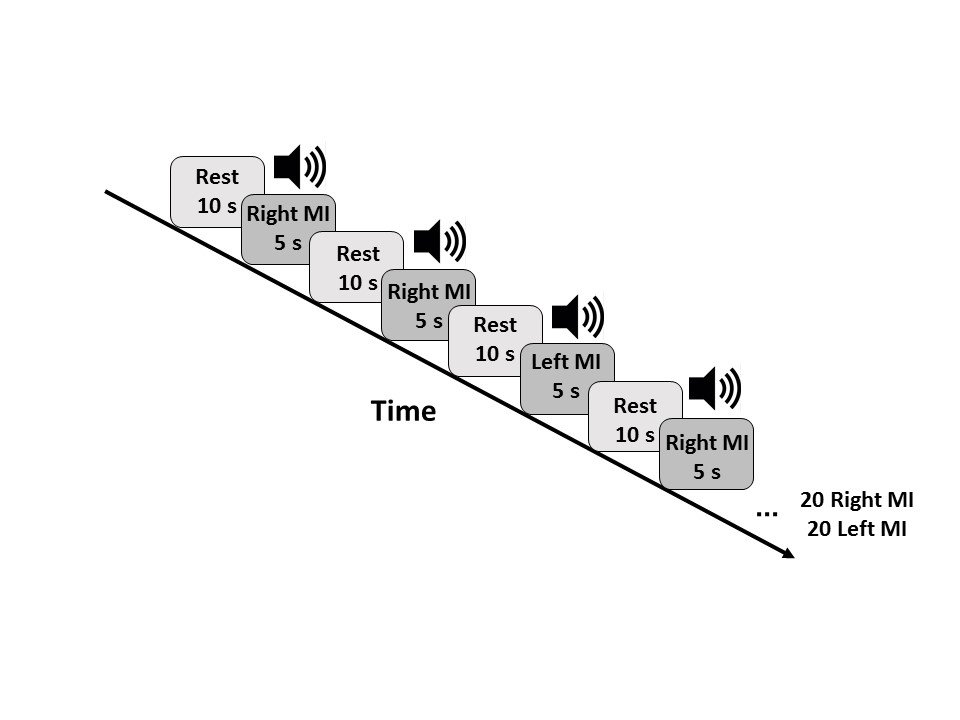
\includegraphics[width=\linewidth]{Slide1.JPG}
	\caption{}
	\label{fig:fig1}
\end{figure}

\section{Methods}
\subsection{Experimental Paradigm}
Six healthy subjects (males, average age of $34 years\pm 5 years$) were recruited for the study. All subjects were right handed, reported no history of neurological or psychiatric disease and did not receive psychoactive medications. 
Subjects set on a chair with the arms comfortably resting on a desk and were asked to perform right or left hand squeezing imagery guided by an acoustic stimulus. The motor imagery task sequence is depicted in figure \ref{fig:fig2}. The 
squeezing imagery consisted of 5 seconds of task and 10 seconds of rest. Right or Left imagery instruction was presented in a pseudo-random order.  During the 5 seconds of task, the subjects were instructed to perform the squeezing imagery with a repetition frequency of $\sim1Hz$. The task provided a total number of 20 Left-hand and 20 Right-Hand 5 seconds trials. 

\begin{figure}
	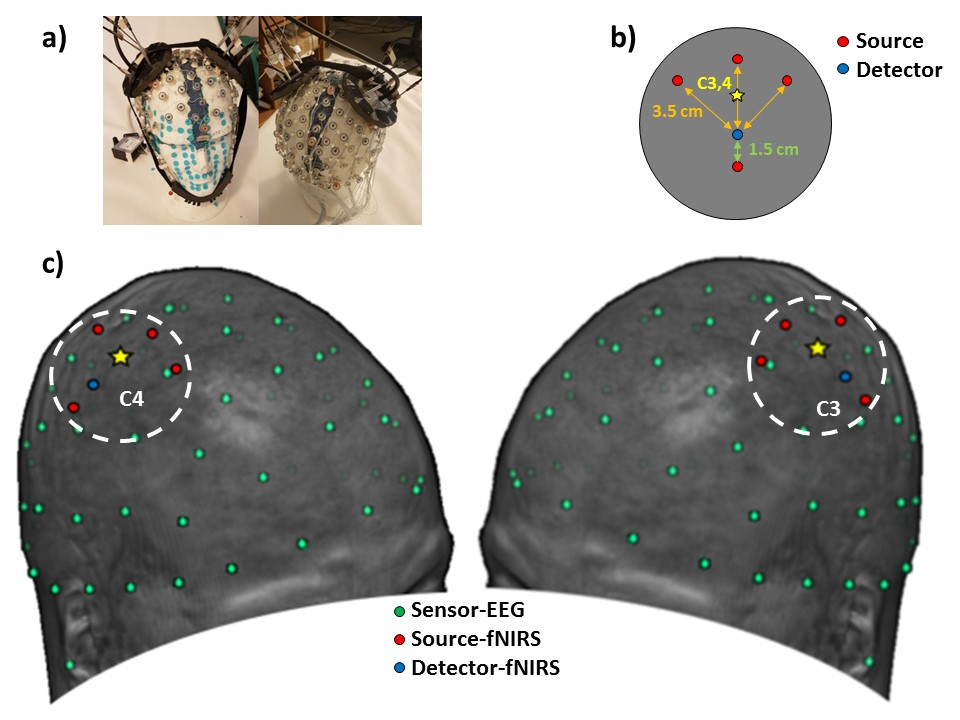
\includegraphics[width=\linewidth]{Slide2.JPG}
	\caption{}
	\label{fig:fig2}
\end{figure}


\subsection{ElectroEncephalography Recordings}
Brain electric activity was recorded with a full-head 128 channels EEG system (Electrical Geodesic Inc, EEG System Net 300, figure \ref{fig:fig1}a,c.).
Skin/electrode impedance was measured before recordings and kept below $50 k\Omega$. EEG data were sampled at 250 Hz and processed in a real time fashion.  Raw data were stored over 1 second window and filtered between 13 Hz and 30 Hz (2nd order Digital Butterworth filter). The beta-band filtered signal was squared and averaged over the second ($\beta_{Pow}$).
 The Event-Related Synchronizations (ERSs) or Event-Related Desynchronizations (ERDs) (Pfurtscheller and Lopes da Silva, 1999; Neuper and Pfurtscheller, 2001) were obtained as relative changes in power during the motor imagery execution with respect to rest:

\begin{equation}
\label{eqn:erders}
ERD/ERS=\frac{\beta_{PowMI}-\beta_{PowBas}}{\beta_{PowBas}}
\end{equation} 
where $\beta_{PowMI}$ is the average power over 1 second window during the task and $\beta_{PowBas}$ is the average power in a 1 second window prior to the task onset.
ERD/ERS values for each second during the task were fed to the learning algorithms for classification. Only 123 of the 128 EEG electrodes were employed in the learning process (5 auxiliary signal electrodes were removed).



\subsection{functional Near Infared Spectroscopy Recordings}
Brain hemodynamic activity was recorded over the sensorimotor regions (C3 and C4, 10-20 System) employing a commercial NIR spectrometer from ISS (Imagent™, Champaign, Illinois).
The apparatus is a Frequency Domain system equipped with 32 laser diodes ($\sim$1 mW  power, 16 emitting light at 690 nm and 16 at 830 nm) and 4 photo-multiplier tubes (PMTs). 
8 light sources (4 injection point, 2 wavelengths) and 1 detectors were employed for each hemisphere. Time-multiplexing was employed for source coding with a total system sampling frequency of 10 Hz.  Light was sent to the scalp using multimodal optical fibers (0.4 mm core) and from the scalp back to the PMTs using fiber bundles (3 mm diameter).  The fibers were held in place using soft, but rigid, custom-built optical patches located on top of the EEG, figure \ref{fig:fig1}a, with an optical layout reported in figure \ref{fig:fig1}b, c. The optical layout consisted of 3 fNIRS channels over C3 and C4 with an interoptode distance (3.5 cm) that allowed sensitivity to brain activity. One short distance channel (1.5 cm),  not sensitive to brain activity (its sensitivity pattern does not reach the brain cortex), provided information regarding scalp-related hemodynamic oscillations (ref.).  
The raw Continuous Wave intensity ($I$)  was averaged  at a 1 sec pace .
The optical densities (ODs)over time were computed as:
\begin{equation}
\label{eqn:erders}
OD=-\ln\frac{I(t)}{I(t_{0})}
\end{equation} 
where $I(t)$ is the signal intensity at second t and $I(t_{0})$ is the average signal intensity in the first second of recording.
Variations in the concentration of oxy-hemoglobin and deoxy-hemoglobin were derived for each channel  based on the Modified Lambert Beer Law [REF.]:

\begin{equation}
\begin{bmatrix}
O_2Hb\\
HHb
\end{bmatrix}
=
\frac{1}{\rho}\begin{bmatrix}
\epsilon_{O_2Hb}(\lambda_1)\cdot DPF(\lambda_1)&\epsilon_{HHb}(\lambda_1)\cdot DPF(\lambda_1)\\
\epsilon_{O_2Hb}(\lambda_2)\cdot DPF(\lambda_2)&\epsilon_{HHb}(\lambda_2)\cdot DPF(\lambda_2)
\end{bmatrix}^{-1}\times
\begin{bmatrix}
OD(\lambda_1)&\\
OD(\lambda_2)
\end{bmatrix}
.
\end{equation}

where $O_{2}Hb$ and HHb represent the changes in oxy-hemoglobin and deoxy-hemoglobin concentrations , $\rho$ is the interoptode distance, $\epsilon$  and DPF are, respectively, the extinction coefficients for the two chromophores and the Differential Pathlength Factors at the wavelengths of interest ($\lambda _{1}$ and $\lambda _{2}$). The extinction coefficients of the two forms of hemoglobin at the different wavelengths  were extracted from Zijlstra et al.[ref.] ( $\epsilon_{O_{2}Hb}(690nm)$ = 0.0096 $mm^{-1}$, $\epsilon_{O_{2}Hb}(830nm)$ = 0.021 $mm^{-1}$, $\epsilon_{HHb}(690nm)$ = 0.05 $mm^{-1}$, $\epsilon_{HHb}(830nm)$ = 0.017 $mm^{-1}$).  The DPFs were derived fron Scholkmann and Wolf  ( $DPF(690nm)$ = 6.5, $DPF(830nm)$ = 5.5) [REF.].
Oxy-hemoglobin $\Delta O_{2}Hb$ and deoxy-hemoglobin $\Delta HHb$ changes during the motor imagery were obtained  with respect to rest (8 channels and 2 Hemoglobin forms for a total of 16 features per second):

 

\begin{equation}
\begin{bmatrix}
\Delta O_2Hb\\
\Delta HHb
\end{bmatrix}
=
\begin{bmatrix}
O_2Hb_{MI}-O_2Hb_{Bas}\\
HHb_{MI}-HHb_{Bas}
\end{bmatrix}
.
\end{equation}
where $O_{2}Hb_{MI}$ and $HHb_{MI}$ are the average hemoglobin concentrations over 1 second window during the task and $O_{2}Hb_{Bas}$ and $HHb_{Bas}$ are the average hemoglobin concentrations in a 1 second window prior to the task onset.
Hemoglobin change  in both short and long distance channels for each second during the task were fed to the learning algorithms for classification. 

\begin{figure}
	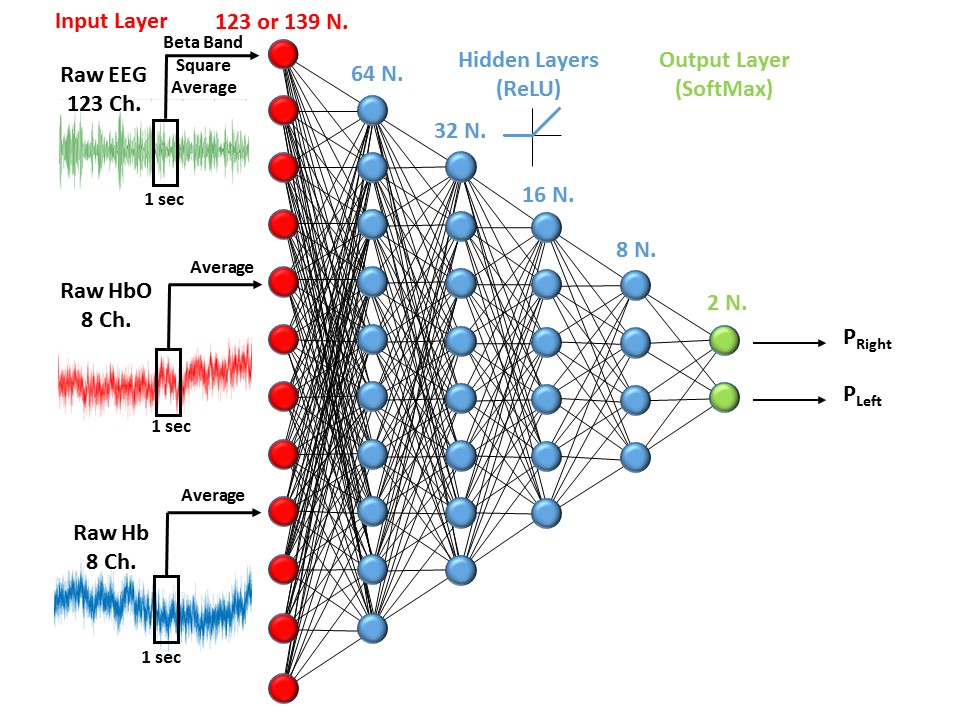
\includegraphics[width=\linewidth]{Slide3.JPG}
	\caption{}
	\label{fig:fig3}
\end{figure}

\subsection{Deep Neural Networks}
Deep Neural Networks (DNNs) allow computational models that are composed of multiple  processing layers composed on non-linear units, called neurons, able to learn representations of data with multiple levels of abstraction.
Deep Neural Networks find complex structure in  data-sets by using the backpropagation algorithm [REF] that guides changes in Networks' parameters that are sequentially updated in each layer from the representation in the previous layer.
Whereas Network parameters are learned from the data, the DNN structure have to be heuristically selected a priori.
Since we performed a first investigatory comparison between DNN performance and other classifier performances, we decided to fix the DNN structure (also called the DNN hyperparameters), without investigating multiple DNN architectures.
The DNN structure employed is presented in figure \ref{fig:fig3}
Our data set consisted of 123 (when standalone EEG classification was performed), or 139 (when both EEG and fNIRS were employed) input neurons. The input neurons feed the EEG and/or the fNIRS feature to the  hidden layers.
Each neuron of the hidden layers perform a non-linear transformation of a linear combination of all the output from the previous layer (full-connected DNN). As a non-linear processing function we decided to employ the Rectified Linear Unit (ReLU) function, which was proven to dampen the vanishing gradient problem providing better performance than other non-linear function (such as the hyperbolic tangent or the sigmoid function) [Ref.]. Hidden neurons operation when ReLU is employed can be written as:

\begin{equation}
y=
\begin{cases}
0,& \text{if } wx+b \leq 0\\
wx+b,&\text{if } wx+b > 0
\end{cases}
\end{equation}


Since the classifier had to discriminate between two states, namely Left or Right Motor Imagery state, the output layer was composed of two neurons performing a softmax transformation:

\begin{equation}
\begin{bmatrix}
P_{Right}\\
P_{Left}
\end{bmatrix}
=
\begin{bmatrix}
\frac{e^{x^Tw_1}}{\sum\limits_{k=1}^2 e^{x^Tw_k}}\\
\frac{e^{x^Tw_2}}{\sum\limits_{k=1}^2 e^{x^Tw_k}}
\end{bmatrix}
.
\end{equation}

The softmax function outputs for the two neurons  the predicted probability of being in the right ($P_{Right}$) or left ($P_{Left}$) imagery state. The number of hidden layers (4) and neurons (refer to figure \ref{fig:fig3}) were selected to approximately decrease ( compress information) the number of processing unit by a factor of 2 between successive layers. 

Weights initialization why

The DNN was trained in a supervised learning approach [REF.].
In the supervised learning, DNN parameters, i.e. weights $w$s and biases $b$s, are adjusted relying on an objective function minimization procedure. The objective function measures the error (or distance) between the output scores and the desired scores . We employed the cross-entropy error as objective function.
Cross-entropy (CE) is defined as:

\begin{equation}
CE=
-\sum \limits_i y'_{i}\ln y_{i}
\end{equation}

where $y$ is the output vector of the DNN ([$P_{Right}$  $P_{Left}$] in the study) $y'$ is the known state ([1 0] for Right Hand Imagery or [0 1] for Left Hand Imagery)
 Cross-entropy metric takes into account the closeness of a prediction and is a more granular way to compute error than Classification Error or Mean Squared Error [Ref.] .
 
Adam Optimizer

Iterations

cross-validation

 learning algorithm,  iterations, cross-validation,  accuracy, software Tensorflow
 
 The described DNN architecture, training and validation were implemented in Python  through the open-source software library Tensorflow [REF.].

\subsection{Post Processing and Statistical Analysis}
Brief introduction of LDA and SVM.
Two way anova recordings-classification.


\begin{figure}
	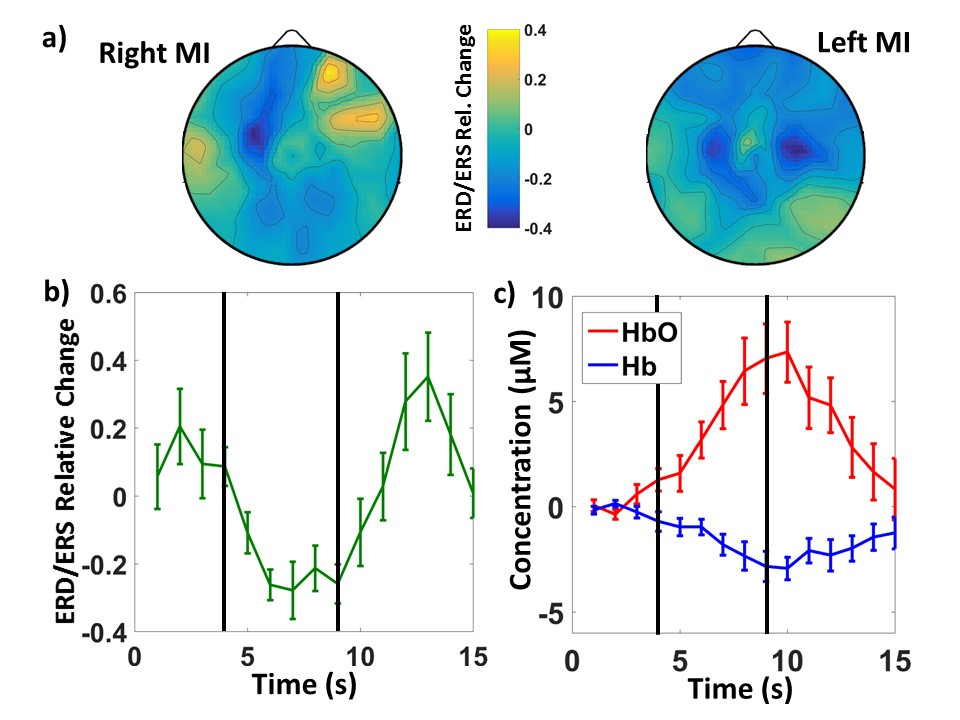
\includegraphics[width=\linewidth]{Slide4.JPG}
	\caption{}
	\label{fig:fig4}
\end{figure}
\begin{figure}
	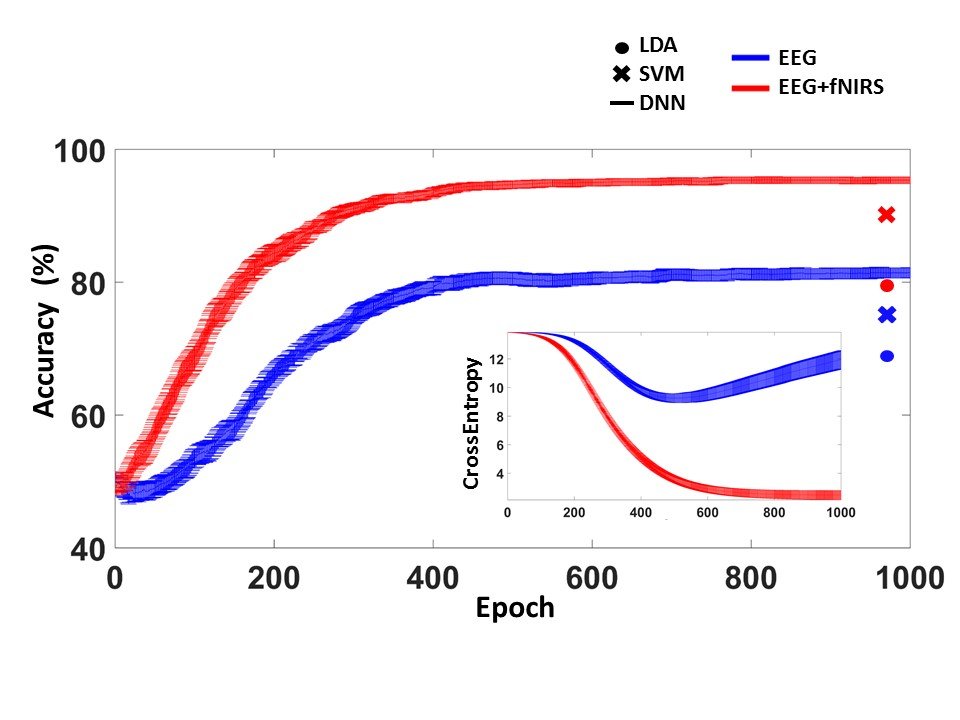
\includegraphics[width=\linewidth]{Slide5.JPG}
	\caption{}
	\label{fig:fig5}
\end{figure}
\begin{figure}
	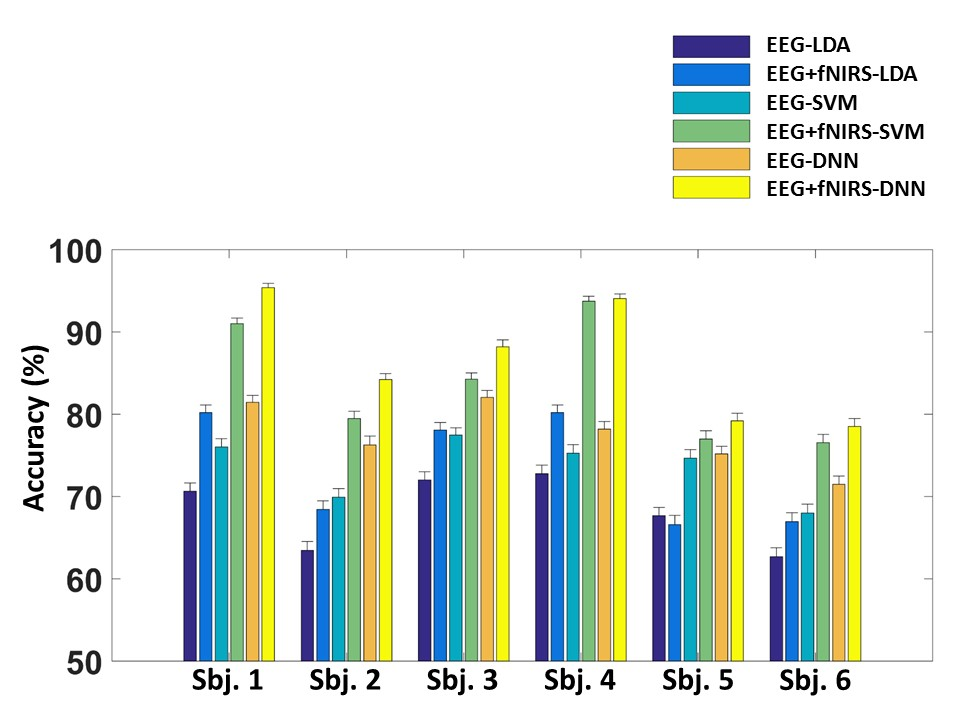
\includegraphics[width=\linewidth]{Slide6.JPG}
	\caption{}
	\label{fig:fig6}
\end{figure}

\subsection{}
\section{Results}
The ERD/ERS time course of beta power for a representative subject is depicted in figure \ref{fig:fig4}b.
Example of average maps-timecourses.
Example of learning curve.
Best performance for DNN
Report overall Performances.
Two way anova SVM DNN of accuracy with respect to EEG-LDA.
Post hoc comparisons.

\section{Discussion}
Short re-caption of main DNN concepts and EEG-fNIRS for MI.
Discussion of obtained results:
increased performance with fNIRS and with DNN classification without interaction (cumulative effect).
Limitations: fixed hyperparameters
(overall length of experiment, frequency band, response time (1sec), DNN structure). 
Report CNN results were poorer (low spatial information content of EEG), may work better with full-head fNIRS.
Future direction RNN for self paced






\section{Conclusion}

\section{Acknowledgements}
This study was partially funded by grant: H2020, ECSEL-04-2015-Smart Health, Advancing Smart Optical Imaging and Sensing for Health (ASTONISH).
 


\end{document}
\newpage
\printbibliography
%\cleardoublepage
%\addcontentsline{toc}{section}{\refname}